\documentclass[11pt,a4paper]{article}
\usepackage[margin=2.3cm]{geometry}
\usepackage[T1]{fontenc}
\usepackage{textcomp}
\input{glyphtounicode}
\pdfgentounicode=1
\usepackage{lmodern}
\usepackage{amsmath}
\usepackage{xcolor}
\usepackage{listings}
\usepackage{tcolorbox}
\tcbuselibrary{breakable}
\usepackage{booktabs}
\usepackage{array}
\usepackage{tikz}
\usetikzlibrary{decorations.pathreplacing}
\usepackage{float}
\usepackage{graphicx}
\graphicspath{{images/}}
\usepackage{hyperref}
\hypersetup{colorlinks=true, linkcolor=blue!50!black, citecolor=green!40!black}

\usepackage{accsupp}
% line numbers are drawn but excluded from copied text
\newcommand{\nocopy}[1]{\BeginAccSupp{method=escape,ActualText={}}#1\EndAccSupp{}}
\lstset{
  language=C, basicstyle=\ttfamily\small, keywordstyle={}, commentstyle={}, stringstyle={},
  numbers=left, numberstyle=\footnotesize\nocopy, numbersep=10pt, xleftmargin=2.4em,
  frame=none, columns=fullflexible, keepspaces=true, upquote=true, showstringspaces=false,
  breaklines=true, captionpos=b, aboveskip=1em, belowskip=0.8em
}
\lstdefinestyle{sh}{language=bash, numbers=none, xleftmargin=2.4em}
\renewcommand{\lstlistingname}{Listing}
% code names in the text: grey monospace
\let\origtexttt\texttt
\renewcommand{\texttt}[1]{\textcolor{black!60}{\origtexttt{#1}}}

\newtcolorbox{keyidea}{colback=blue!4, colframe=blue!45!black, title=Key ideas, fonttitle=\bfseries\small}
\newtcolorbox{experiment}{breakable, colback=orange!5, colframe=orange!70!black, title=Experiment, fonttitle=\bfseries\small}
\title{\textbf{OpenMP GPU Functions and Globals: \texttt{declare target}}\\[4pt]\large Lesson 204: calling your own functions inside a GPU kernel}
\author{Gustavo Lozano}
\date{November 2026}

\begin{document}
\maketitle

\noindent\textit{\small Source: Deakin \& Mattson~\cite{dm}, Appendix A.2 (Directives and
Constructs for the GPU). Prerequisite: \texttt{00-openmp\_target\_data.pdf} (Lesson 201).}

\section{The idea}
The GPU runs its own machine code. A function called inside a \texttt{target} region must
therefore exist in a \emph{device version}, and a global variable it uses must have a
\emph{device copy}. \texttt{declare target} asks the compiler for both:
\begin{lstlisting}[numbers=none]
#pragma omp declare target
double scale = 2.0;        /* a host copy and a device copy  */
double f(double x) { ... } /* a host version and a device version */
#pragma omp end declare target
\end{lstlisting}

The two copies of \texttt{scale} are separate variables (Figure~\ref{fig:copies}). The device
copy starts with the initial value, $2.0$. After that, changing the host copy does not change the
device copy: \texttt{target update to(scale)} copies it, as in Lesson 201.

\begin{figure}[H]
\centering
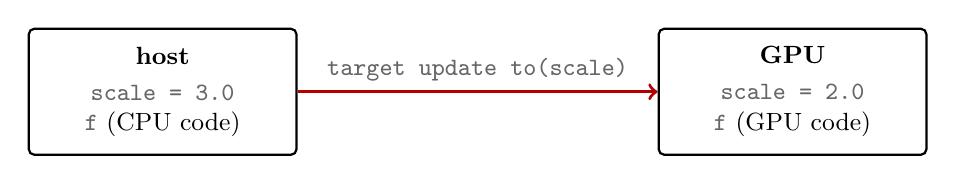
\begin{tikzpicture}[font=\small, box/.style={draw, thick, rounded corners=2pt, minimum
  width=3.4cm, minimum height=1.6cm, align=center}]
  \node[box] (h) at (0,0) {\textbf{host}\\[2pt] \texttt{scale = 3.0}\\ \texttt{f} (CPU code)};
  \node[box] (d) at (8,0) {\textbf{GPU}\\[2pt] \texttt{scale = 2.0}\\ \texttt{f} (GPU code)};
  \draw[->, very thick, red!70!black] (h.east) -- node[above] {\texttt{target update to(scale)}}
     (d.west);
\end{tikzpicture}
\caption{After \texttt{scale = 3.0} on the host, the GPU still sees $2.0$ until
\texttt{target update to(scale)} copies the new value.}
\label{fig:copies}
\end{figure}

\paragraph{Is it always needed?} Clang creates a device version of a function it can see in the
same file and that is called in a \texttt{target} region, even without the directive. It is
needed for a function defined in \emph{another file}, and for a \emph{global variable}: without
it there is no device copy of \texttt{scale} to read.

\section{The code}
\texttt{f} and \texttt{scale} are in a \texttt{declare target} block (lines 20--27).
\texttt{apply\_gpu} computes \texttt{y[i] = f(x[i])} on the GPU, and \texttt{check} compares the
result with \texttt{f} on the host, which uses the host copy of \texttt{scale}. The program runs
the kernel three times:
\begin{enumerate}
  \item with the initial \texttt{scale = 2.0};
  \item after \texttt{scale = 3.0} on the host (line 63);
  \item after \texttt{target update to(scale)} (line 67).
\end{enumerate}

\begin{lstlisting}[caption={\textbf{\origtexttt{declare\_target.c}} -- a function and a global variable on the GPU with \origtexttt{declare target}.}, label={lst:dt}]
/*
 * declare_target.c -- OpenMP Lesson 204: functions and global variables on
 * the GPU with declare target.
 * Source: Deakin & Mattson (2023), Appendix A.2 (Directives and Constructs
 *         for the GPU).
 *
 * f(x) = scale * x * x + 1 is called inside a GPU kernel.  f and the global
 * variable scale are in a declare target block, so the compiler builds a
 * device version of f and keeps a device copy of scale.
 *
 * Compile:  clang -O2 -fopenmp --offload-arch=sm_61 \
 *                 -o declare_target declare_target.c
 * Run:      OMP_TARGET_OFFLOAD=MANDATORY ./declare_target
 */

#include <stdio.h>
#include <stdlib.h>
#include <omp.h>

#pragma omp declare target
double scale = 2.0;                    /* one copy on the host, one on the GPU */

double f(double x)                     /* compiled for the host and the GPU    */
{
    return scale * x * x + 1.0;
}
#pragma omp end declare target

/* y[i] = f(x[i]) on the GPU */
static void apply_gpu(const double *x, double *y, long n)
{
    #pragma omp target teams distribute parallel for \
            map(to: x[0:n]) map(from: y[0:n])
    for (long i = 0; i < n; i++)
        y[i] = f(x[i]);
}

/* compare with f on the host, which uses the host copy of scale */
static void check(const char *step, const double *x, const double *y, long n)
{
    long bad = 0;
    for (long i = 0; i < n; i++)
        bad += (y[i] != f(x[i]));
    printf("%-34s host scale = %.1f   y[1] = %5.1f   correct: %s\n",
           step, scale, y[1], bad ? "NO" : "yes");
}

int main(void)
{
    long n = 1L << 20;
    double *x = malloc(n * sizeof(double));
    double *y = malloc(n * sizeof(double));
    for (long i = 0; i < n; i++) x[i] = (double)(i % 8);

    int on_host = 1;
    #pragma omp target map(from: on_host)
    on_host = omp_is_initial_device();
    printf("kernels run on: %s\n", on_host ? "CPU" : "GPU");

    apply_gpu(x, y, n);
    check("1. first kernel:", x, y, n);

    scale = 3.0;                       /* changes only the host copy */
    apply_gpu(x, y, n);
    check("2. scale = 3 on the host:", x, y, n);

    #pragma omp target update to(scale)
    apply_gpu(x, y, n);
    check("3. after target update to(scale):", x, y, n);

    free(x); free(y);
    return 0;
}
\end{lstlisting}

\begin{lstlisting}[style=sh]
clang -O2 -fopenmp --offload-arch=sm_61 -o declare_target declare_target.c
OMP_TARGET_OFFLOAD=MANDATORY ./declare_target
\end{lstlisting}

\begin{keyidea}
\begin{itemize}
  \item \texttt{declare target} builds a device version of a function and a device copy of a
        global variable.
  \item The host and device copies of a global are separate; \texttt{target update} keeps them
        in step.
  \item Functions in other files and global variables need the directive explicitly.
\end{itemize}
\end{keyidea}

\section{The experiment}
\begin{experiment}
\textbf{Question:} when does the GPU see a new value of a global variable?

Run the program on the GPU, and then with offloading disabled:
\begin{lstlisting}[style=sh]
OMP_TARGET_OFFLOAD=MANDATORY ./declare_target
OMP_TARGET_OFFLOAD=DISABLED  ./declare_target
\end{lstlisting}

\textbf{What to observe and answer.}
\begin{enumerate}
  \item On the GPU, which step is wrong? What value of \texttt{scale} did the kernel use there?
        (Hint: for \texttt{x[1] = 1}, $f(1) = \texttt{scale} + 1$.)
  \item Why is every step correct when offloading is disabled?
  \item Remove line 67. Which steps are wrong now?
\end{enumerate}
\end{experiment}

\paragraph{Answers (read after trying).}

\noindent(1)~Step 2: \texttt{y[1]} is $3.0$, so the kernel used \texttt{scale} $= 2.0$, the
device copy, while the host compares with $3.0 + 1 = 4.0$. Step 3 is correct again because
\texttt{target update to(scale)} copied $3.0$ to the GPU.

\noindent(2)~With \texttt{DISABLED} the kernels run on the host, and the host has only one
\texttt{scale}: there is no second copy to get out of step.

\noindent(3)~Steps 2 and 3: the GPU keeps using $2.0$ for the rest of the program.

\paragraph{Next lesson.} Lesson 205: the \texttt{loop} construct, a simpler way to write GPU
loops.

\begin{thebibliography}{9}
\bibitem{dm} T.~Deakin and T.~G.~Mattson. \emph{Programming Your GPU with OpenMP: Performance
  Portability for GPUs}. MIT Press, Cambridge, MA, 2023.
\end{thebibliography}
\end{document}
